%%%%%%%%%%%%%%%%%%%%%%%%%%%%%%%%%%%%%%%%%%%%%%%%%%%%%%%%%%%%%%%%%%%%%%
%%  dissertation.tex, to be compiled with latex2e.                   %
%%  16 April 2012                                                    %
%%%%%%%%%%%%%%%%%%%%%%%%%%%%%%%%%%%%%%%%%%%%%%%%%%%%%%%%%%%%%%%%%%%%%%
%%                                                                   %
%%  Writing a Doctoral Dissertation with LaTeX at                    %
%%           Georgia State University                                %
%%                                                                   %
%%  (Running this ``template'' will generate the documentation.)     %
%%                                                                   %
%%%%%%%%%%%%%%%%%%%%%%%%%%%%%%%%%%%%%%%%%%%%%%%%%%%%%%%%%%%%%%%%%%%%%%
 
%\documentclass[12pt,gsu,online,openright,doubleside]{gsudiss}
\documentclass[12pt,gsu,online,openany,singleside,hidelinks]{gsudiss}
% \usepackage[square, numbers]{natbib}
%\usepackage{subfigure}                % To format bibliographies.
%% \usepackage{aastex}
\bibliographystyle{siam}
% \setlength{\bibsep}{0pt}           % Necessary for bib entries to have
%                                    % correct line spacing.
\usepackage{tocloft}
\usepackage[hidelinks]{hyperref}
\usepackage{mathtools}
\usepackage{todonotes}
\usepackage{subcaption}
\captionsetup[subfigure]{labelformat=simple}
\renewcommand{\thesubfigure}{(\alph{subfigure})}

\usepackage[commentmarkup=footnote]{changes}
\definechangesauthor[name=MS]{MS}
% \def\comm#1{\added[comment={#1}]{}}
\newcommand{\comm}[1]{\added[comment={#1}]{}}
\newcommand{\del}[1]{\deleted[comment={remove}]{#1}}
\newcommand{\rep}[2]{\replaced{#1}{#2}}
\def\vec#1{\mathbf{#1}} % \newcommand won't override existing definitions.
\def\eqand{\qquad\text{and}\qquad}
\hypersetup{
    colorlinks=false,
    pdfborder={0 0 0},
}
%%%%%%%%%%%%%

\renewcommand{\cftfigfont}{Figure\ }
\renewcommand{\cfttabfont}{Table\ }
\renewcommand{\cftchapfont}{\bfseries}
\renewcommand{\cftsecfont}{\bfseries}
\renewcommand{\cftsubsecfont}{\bfseries\itshape}
\renewcommand{\cftsubsubsecfont}{\itshape}
\renewcommand{\cftparafont}{\mdseries}

\usepackage{lscape}
\usepackage{geometry}
\usepackage{array}
% \usepackage{deluxetable}
%\usepackage{aastex_hack}
% \usepackage{longtable,ltcaption}
\usepackage{float}
% \usepackage[caption = false]{subfig}
% The ltcaption package supports \CaptionLabelFont & \CaptionTextFont
% introduced by the NTG document classes
%\renewcommand\CaptionLabelFont{\normalsize}
%\renewcommand\CaptionTextFont{\normalsize}

% \usepackage{aas}                   % Some abbreviations for AAS references.
% \citestyle{aa}                     % Astronomy & Astrophysics cite style.


\usepackage{eucal}                 % Euler fonts for equations.
\usepackage{verbatim}              % Allows quoting source with commands.
\usepackage{graphicx}              % For powerful manipulation of figures.
\usepackage{ragged2e}
\usepackage{algorithm}
\usepackage{float}
\usepackage{algpseudocode}
\usepackage{amsmath,amsthm,amsfonts,amsopn,amssymb} % Some nice math packages.
% \usepackage{ctable}                % My preference table package.
\usepackage[overlay]{textpos}      % Put stuff anywhere, I mean anywhere ...
\usepackage{pstricks}              % Draw stuff especially on top figures etc...
\usepackage{afterpage}             % Useful for absolute placement of figures and tables.
\usepackage{longtable} % for 'longtable' environment
\usepackage{pdflscape} % for 'landscape' environment

%\input{figures}                    % My defined figures, see the file "figures.tex".
\newcommand\arcdeg{\mbox{\ensuremath{^\circ}}}%
\newcommand\arcmin{\mbox{\ensuremath{^\prime}}}%
\newcommand\arcsec{\mbox{\ensuremath{^{\prime\prime}}}}%
\newcommand{\point}{\mbox{\ensuremath{\!\!.}\thinspace}}
\newcommand{\minusone}{\ensuremath{^{-1}}}
\newcommand{\minustwo}{\ensuremath{^{-2}}}
\newcommand{\minusthree}{\ensuremath{^{-3}}}
\newcommand{\minusfive}{\ensuremath{^{-5}}}
\newcommand{\plusthree}{\ensuremath{^{3}}}
\newcommand{\plusfive}{\ensuremath{^{5}}}
\newcommand{\kms}{\mbox{\ km\,s\ensuremath{^{-1}}}}
\newcommand{\fig}{Figure~}
\newcommand{\figs}{Figures~}
\newcommand{\tab}{Table~}
\newcommand{\tabs}{Tables~}
\newcommand{\eqn}{Equation~}
\newcommand{\eqns}{Equations~}
\newcommand{\vracc}{\mbox{$\mathrm{v=kr}$}\xspace}
\newcommand{\vrdec}{\mbox{$\mathrm{v=v_{max}-k^{'}(r-r_t)}$}\xspace}
\newcommand{\vrootracc}{\mbox{$\mathrm{v=k_{1}\sqrt r}$}\xspace}
\newcommand{\vrootrdec}{\mbox{$\mathrm{v=v_{max}-k_{2}\sqrt{r-r_t}}$}\xspace}
\newcommand{\rlaw}{\mbox{$r\ $law}\xspace}
\newcommand{\rootrlaw}{\mbox{$\sqrt r\ $law}\xspace}
\newcommand{\resolvingpower}{\mbox{$\lambda/\Delta\lambda$}\xspace}
\newcommand{\OIII}{\mbox{[\acs{O3}]}\xspace}
\newcommand{\solarmass}{\mbox{\ M\ensuremath{_{\odot}}}}
\newcommand{\arcpt}{${{\lower3pt\hbox{$^{\prime\prime}$}}\atop{\raise4pt\hbox{.}}}$}
\newcommand{\msun}{$M_\odot$}               % User defined commands go in this
                                   % file called "usercommands.tex".
                                   % Of course you can rename it.
\usepackage{float}
\floatstyle{boxed}
\newfloat{code}{h}{ext}
\floatname{code}{Code}


\usepackage{fancyvrb}
\DefineVerbatimEnvironment{code}{Verbatim}{fontsize=\small}
\DefineVerbatimEnvironment{example}{Verbatim}{fontsize=\small}

\newtheorem{theorem}{Theorem}[section]
\newtheorem{definition}{Definition}[section]
\newtheorem{corollary}{Corollary}[theorem]
\newtheorem{lemma}[theorem]{Lemma}





\usepackage{atbeginend}            % Modify space before and after
                                   % equations. These are my preferences.
\AfterBegin{equation}{\addtolength{\abovedisplayskip}{-0.5\baselineskip}}
\BeforeEnd{equation}{\addtolength{\belowdisplayskip}{-0.5\baselineskip}}
\AfterBegin{equation*}{\addtolength{\abovedisplayskip}{-0.5\baselineskip}}
\BeforeEnd{equation*}{\addtolength{\belowdisplayskip}{-0.5\baselineskip}}

\renewcommand{\topfraction}{0.85}        % These modify figure placement on
% \renewcommand{\bottomfraction}{0.85}     % the page and various other space
\renewcommand{\textfraction}{0.10}       % requirements for figures.
\renewcommand{\floatpagefraction}{0.80}  % These 5 lines are not
\renewcommand{\arraystretch}{0.5}        % necessary but I think its better
                                         % than latex default.

\setlength{\tabcolsep}{3pt}        % shrink column spacing so your tables 
                                   % can be wider (yay Todd Tables)
%\setlength{\LTcapwidth}{\textwidth}% so your rotated, normal-sized
                                   % longtable titles won't wrap oddly.



\clubpenalty=1000                  % Make Latex try hard to fix
\widowpenalty=1000                 % "stray lines" in paragraphs,
                                   % i.e. paragraph that begin at the
                                   % last line of a page, or end with
                                   % the last line on the following
                                   % page. This looks silly.
\raggedbottom

\settocname{TABLE OF CONTENTS}              % Set the "Table of Contents"
                                   % name. This is the default. You
                                   % can use "Table of Contents" for example.

\setlofname{LIST OF FIGURES}               % Change the name from 'List of
                                   % Figures'. Use whatever you wish.

\setlotname{LIST OF TABLES}                % Change the name from 'List of
                                   % Tables'. Use whatever suit your
                                   % fancy.

\settocbibname{REFERENCES}         % Change the name from
                                   % 'Bibliography'. Change it back if
                                   % you feel like it.

\setloaname{LIST OF ABBREVIATIONS}
                                   % I Changed the name from 'List of
                                   % Abbreviations'. Use any name that
                                   % makes sense here. If you don't
                                   % have an "abbreviations.tex" file,
                                   % this command will do nothing.

\setfigname{Figure\ }               % Set the caption labels for figures.

\settabname{Table\ }                % Set the caption labels for tables.

\setcapfont{pnc}                   % Set the caption font for
                                   % both tables and figures.

\chapternumsize{\normalsize}            % You can use any standard latex sizes here.
\chapterheadsize{\normalsize}           % You can use any standard latex sizes here.
\chaptertitlesize{\normalsize}           % You can use any standard latex sizes here.
                                   % These defaults look good to me.

\beforechapterheadname{CHAPTER}         % Optional text to put in front of
                                   % the chapter number.
\afterchapterheadname{}          % Optional text to put after the
                                   % chapter number. The default
                                   % looks like this: --1--. Of course
                                   % you can change this to any
                                   % format, for e.g. $\sim$

\chapterheadpos{center}            % You can use 'right', 'left',
                                   % 'center'.

\chaptertitlepos{center}           % You can use 'right', 'left',
                                   % 'center'

\chapterheadverticalspace{-1em}     % The space between the Chapter head
                                   % and the top of page. This distance
                                   % is not absolute, but relative to
                                   % the parameters set by the
                                   % geometry package. Play around
                                   % with this number to suit your needs.

\chapterbetweentitlespace{-1.em}   % The space between the chapter head
                                   % and the title head.

\titleheadverticalspace{2em}       % The space between the title head
                                   % and the text.

\sectiontitlesize{\normalsize}          % This is obvious.
\sectiontitlepos{left}             % Obvious.

\sectiontitleverticalspace{1em}    % The space between the section head
                                   % and the text.

\subsectiontitlesize{\normalsize}       % Obvious.
\subsectiontitlepos{left}          % Obvious.

\subsectiontitleverticalspace{0.5em} % You get the idea...

\subsubsectiontitlesize{\normalsize}
\subsubsectiontitlepos{left}

\subsubsectiontitleverticalspace{0.5em}

\sepabbrev{7em}                    % The space between the abbreviation
                                   % lists, that is, if you have
                                   % one. Has to be >= 5em.

\prettify{pnc}

\printdraft{\textcolor{gray}\small DRAFT}    % In order to use this
                                   % command, you have to enable "drafts"
                                   % in the option of the gsudiss
                                   % class, otherwise it does
                                   % nothing. This prints the word
                                   % "DRAFT" in gray color in the header of your
                                   % dissertation. You can go wild
                                   % here if you want. Just make sure
                                   % you disable the draft option
                                   % before final printing.

\author(Ayobami Adebesin)              % Name required.

\title(The Spectral Transformation Lanczos Algorithm for the Symmetric-Definite Generalized Eigenvalue Problems: A Comparative Analysis with Conditioning Insights)    % Title of dissertation Required.

\titlesize(11)(11)                               % This is for changing
                                             % the default font size
                                             % for your title. The
                                             % first argument is the
                                             % font size, the second
                                             % is the line spacing for
                                             % long tiles that wrap to
                                             % more than one line.
                                             % Default is equivalent
                                             % to the \LARGE command,
                                             % which is roughly (22)(22).

% \committee: The first parenthesis must contain your supervisor name.
%         You can have two supervisors, in which case, the
%         second supervisor goes into the square brackets, next to the
%         first. If you have one like me, then leave the second entry blank, like below. The
%         rest of the parentheses contains the rest of your committee members. You
%         can have up to six entries, NOT including your supervisor(s). My
%         school requires five or four. I have five (5) members
%         below. Note that there is no need to put the "Dr." title in front of any of the names.
% Adjust margins to 1.0in on all sides

\committee(Michael Stewart)[]
          (Russell Jeter)
          (Vladimir Bondarenko)
          (\qquad)
          (\qquad)

\department(Department of Mathematics and Statistics)
                                   % Your Department name.
                                   % Other departments you can
                                   % use include
                                   % \department(School of Arts \& Design)
                                   % or \department(School of Music), etc...

\departmenttitle(Chair)            % For Arts and Music school
                                   % students use
                                   % \departmenttitle{Director}

\graduationyear(2025)              % Defaults to the same year
                                   % you are writing this
                                   % Dissertation. Do
                                   % \graduationyear(200x) if
                                   % you ever need to change it.

\graduationmonth(May)           % This is the date of the
                                   % official graduation ceremony.
                                   % Do \graduationmonth{January}
                                   % for example. Defaults to "August"
\newcommand\omicron{o}

%%%%%%%%%%%%%%%%%%%%%%%%%%%%%%%%%%%%%%%%%%%%%%%%%%%%%%%%%%%%%%%%%%%%%%
%               The dissertation starts here.                        %
%%%%%%%%%%%%%%%%%%%%%%%%%%%%%%%%%%%%%%%%%%%%%%%%%%%%%%%%%%%%%%%%%%%%%%

\begin{document}
\pagestyle{empty}
\begin{center}
%\vspace*{.1in}
\rep{The Spectral Transformation Lanczos Algorithm for the Symmetric-Definite Generalized Eigenvalue Problem: A Comparative Analysis with Conditioning Insights}{Spectral Transformation Lanczos Algorithm for Symmetric-Definite Generalized Eigenvalue Problems: A Comparative Analysis with Conditioning Insights.}

\vspace{.9in}
by\\
\vspace{.9in}
Ayobami Adebesin\\
\vspace{.9in}
Under the Direction of Michael Stewart, Ph.D. \\
\vspace{2in}

A Thesis Submitted in Partial Fulfillment of the Requirements for the Degree of\\  % Choose either thesis or dissertation and delete the other.
\vspace{.2in}
Master of Science \\
\vspace{.2in}
in the College of Arts and Sciences \\
\vspace{.2in}
Georgia State University \\
\vspace{.2in}
2025
\pagebreak 



ABSTRACT\\
\bigskip
\end{center}

\begin{flushleft}
	\justify
	This thesis investigates the application of the spectral transformation Lanczos (ST-Lanczos) algorithm to a dense symmetric-definite generalized eigenvalue problem involving real, symmetric matrices $A$ and $B$, with $B$ being positive definite and possibly\del{,} ill-conditioned. The Lanczos algorithm is a well-known iterative algorithm for computing the eigenvalues of a symmetric matrix and it works well \rep{finding extreme points in the spectrum.}{if the spectrum of the eigenvalues are well-spaced.} By leveraging a shifted and inverted formulation of the problem, the ST-Lanczos algorithm relies on iterative projection to approximate extremal eigenvalues near a shift $\sigma$.   While previous work has been done in using ST-Lanczos for sparse problems, we adapt this technique to dense problems and analyze how the error bounds already proven for direct methods plays out in an iterative context. \comm{Mostly we are testing on dense problems.  I would not say we are adapting it to dense matrices.  We simply happen to use some dense test problems because it is convenient.} \\[10pt]
	This study primarily focuses on benchmarking the ST-Lanczos method against established direct methods in the literature and addresses challenges in numerical stability, computational efficiency, and sensitivity of residuals to ill-conditioning.
\end{flushleft} 
\begin{singlespace}
\vspace{0.5in}
\noindent INDEX WORDS:
\hspace{0.2in}
\parbox[t]{4.5in}{
  eigenvalues, eigenvectors, \rep{Lanczos}{lanczos} algorithm, \rep{Ritz}{ritz} values, \rep{Krylov}{krylov} subspaces, spectral transformation, orthogonality}
\end{singlespace} 
            % See the TitleAbstract.tex file
%%%%%%%%%%%%%%%%%%%% The front matter of your document %%%%%%%%%%%%%%%%%%%%


\frontmatter

\certifypage                 % Produces the certify page, if this option is
                             % set in the class file.



\copyrightpage               % Produces the copyright page.
\clearpage
\approvalpage                % Produces the approval page.
\clearpage
\dedicationpage              % The dedication page is optional.
\clearpage                             % This command does nothing if you don't
                             % have a `dedication.tex' file, otherwise
                             % the file is included in the frontmatter.

\acknowledgmentpage          % The acknowledge page is optional.
\clearpage                             % This command does nothing if you don't
                             % have an `acknowledgment.tex' file, otherwise
                             % the file is included in the frontmatter.

\tableofcontents             % Table of Contents will be automatically
\clearpage                             % generated and placed here.

\listoftables                % List of Tables will be automatically
\clearpage                             % generated if you had made proper table captions.

\listoffigures               % List of Figures will be automatically
\clearpage                             % generated if you had made proper figure captions.

\listofabbreviations         % List of Abbreviations will be
\clearpage                             % automatically generated if you had made any,
                             % following the style of the "Acronym"
                             % package. See my "abbreviation.tex" file
                             % for example usage. If you don't have
                             % this file, the command does nothing.
              % See the frontmatter.tex file

\mainmatter                        % Main chapters starts here
\chapter{INTRODUCTION}
\newtheorem{theorem}{Theorem}[section]
\newtheorem{definition}{Definition}[section]

\section{Background}\label{sec:Background}

The problem of computing eigenvalues and eigenvectors of matrices in numerical linear algebra is a well-studied one. The computation of eigenvalues and eigenvectors plays a central role in scientific computing with applications in structural analysis, quantum mechanics, data science and control theory. However, eigenvalue problems(standard and generalized)  involving dense and sparse matrices present significant computational challenges, especially as the size of the matrices increases. These problems are fundamental in many scientific and engineering disciplines where the underlying mathematical models are often expressed in terms of eigenvalue equations. Historically, methods for solving eigenvalue problems date back to the early 20th century with foundational contributions from David Hilbert, Erhard Schmidt, and John von Neumann, who laid the groundwork for understanding linear operators and their spectral properties.

With the advent of digital computing in the mid-20th century, numerical methods for eigenvalue problems began to flourish. Classical iterative methods, such as the power iteration and inverse iteration, were among the first to be employed due to their simplicity and effectiveness for small-scale problems. However, as computational requirements grew, particularly with the need to solve larger sparse systems, researchers turned to more sophisticated algorithms. The Lanczos method, introduced by Cornelius Lanczos in 1950,
represented a significant advancement for efficiently solving eigenvalue problems for large symmetric matrices. The method exploits the sparsity of matrices and reduces the dimensionality of the problem by constructing a tridiagonal matrix whose eigenvalues approximate those of the original matrix.

An important class of eigenvalue problems which is the main focus of this thesis, is the generalized eigenvalue problem {} (GEP). The GEP takes the form $A\mathbf{v} = \lambda B\mathbf{v}$ where $A$ and $B$ are square matrices, $\lambda$ is a generalized eigenvalue, and $\mathbf{v}\neq\mathbf{0}$ is the corresponding generalized eigenvector. This class of problems arises naturally in a number of application areas, including structural dynamics, data analysis and has a long history in the research literature on numerical linear algebra.

\section{Literature Review}\label{sec:LiteratureReview}
Generalized eigenvalue problems involving symmetric and positive definite matrices are fundamental in numerical linear algebra with applications in structural  dynamics, quantum mechanics, and control theory. Solving these kind of problems involve computing the eigenvalues $\lambda$ and eigenvectors $v$ that satisfies the equation. The choice of method depends on the properties of the matrix involved in the problem we are trying to solve (e.g, sparsity, symmetry) and computational constraints. In this section, we discuss some of the research that has been done on this topic.

\cite{doi:10.1137/1.9781421407944}\comm{Use numbered citations by commenting out some of the astronomical citation style things in the \LaTeX\ preamble.  I suggest adding instead \textbackslash bibliographystyle\{siam\}.  You can diff to see the changes I made to the preamble.  As you have here, don't start a sentence with a reference; numbered references are common in math, but they look weird at the start of a sentence.} considered the case when B\comm{use math mode here} is invertible, in which the problem is reduced to $B^{-1}A\mathbf{v} = \lambda \mathbf{v}$. However, explicity forming $B^{-1}A$ is numerically unstable if B is ill-conditioned. Since $B$ a symmetric and positive definite $B$, one can compute a Cholesky factorization $B = LL^{T}$ which allows us to reduce the equation to a standard eigenvalue problem $L^{-1}AL^{-T}\mathbf{y} = \lambda \mathbf{y}$ where $\mathbf{y}= L^T \mathbf{v}$, which can then be solved by using the symmetric $QR$ algorithm to compute a Schur decomposition.

The $QZ$ algorithm (\cite{5b3d5fb1-4813-3046-9331-a730b392f611}) for the non-symmetric GEP, is an iterative method that generalized the $QR$ algorithm, to handle singular or ill-conditioned $B$. It applies orthogonal transformations to simutaneously reduce $A$ and $B$ to upper triangular forms from which the eigenvalues are extracted. Although this method is robust and backward stable, it is computationally expensive, thereby limiting its use to small or medium sized matrices.

\section{Mathematical Preliminaries}\label{sec:MathPrelim}
In this section, we shall introduce some notations and the key mathematical concepts underlying the eigenvalue problems that will be used throughout this study.
\subsection{Notation}
Throughout this study, we make use of the following notations:
\begin{align*}\nonumber
	&A \in \mathbb{R}^{m\times n}: \text{denotes a matrix}\\
	&[A]_{ij}: \text{denotes element $(i, j)$ of $A$}\\
	&\mathbf{x} \in \mathbb{R}^{m}: \text{denotes a column vector}\\
	&A^{T}: \text{denotes the transpose of matrix $A$}\\
	&\| \cdot \|: \text{denotes a vector or matrix norm }\\
	& \otimes: \text{ denotes the Kronecker product of two matrices}\\
	&A_{i:i^\prime, j:j^\prime}: \text{denotes the $(i^\prime - i + 1) \times (j^\prime - j + 1)$ submatrix of $A$}\\
	&A^{(k)}: \text{denotes the matrix A at the $k$th step of an iteration}
\end{align*}
\subsection{Floating Point Arithmetic}
We define a \textit{floating point} number system, \textbf{F} as a bounded subset of the real numbers $\mathbb{R}$, such that the elements of $\mathbf{F}$ are the number $0$ together with all numbers of the form
\begin{align*}
	x = \pm(m / \beta^t)\beta^e\text{{,}}
\end{align*}
where $m$ is an integer in the range $1\leq m\leq \beta^t$ known as the significand, $\beta \geq 2$ is known as the \textit{base} or \textit{radix} (typically $2$), $e$ is an arbitrary integer known as the exponent and $t\geq 1$ is known as the precision.\\
To ensure that a nonzero element $x \in$ \text{F} is unique, we can restrict the range of \textbf{F} to $\beta^{t-1} \leq m \leq \beta^t - 1$. The quantity $\pm(m/\beta^t)$ is then known as the \textit{fraction} or \textit{mantissa} of x. We define the number $u \coloneq \frac{1}{2}\beta^{1-t}$ as the \textit{unit roundoff} or \textit{machine epsilon}. In a relative sense, the \textit{unit roundoff} is as large as the gaps between floating point numbers get.\\
Let $fl :  \mathbb{R} \rightarrow \mathbf{F}$ be a function that gives the closest floating point approximation to a real number, then the following theorem gives a property of the unit roundoff.
\begin{theorem}
	If $x \in \mathbb{R}$ is in the range of $\mathbf{F}$, then $\exists$ $\epsilon$ with $|\epsilon| \le u$ such that $fl(x) = x(1+\epsilon)$.
\end{theorem}
One way we could think of this is that, the difference between a real number and its closest floating point approximation is always smaller than $u$ in relative terms.

\subsection{Conditioning and Stability}\label{sec:ConditioningAndStability}
Given any mathematical problem $f: X \rightarrow Y$, the conditioning of that problem pertains to the perturbation behaviour of the problem, while stability of the problem pertains to the perturbation behaviour of an algorithm used in solving that problem on a computer. A \textit{well-conditioned} problem is one with the property that small perturbations of the input lead to only small changes in the output. An \textit{ill-conditioned} problem is one with the property that small perturbations in the input leads to a large change in the output.

For any mathematical problem, we can associate a number called the \textit{condition number} to that problem that tells us how well-conditioned or ill-conditioned the problem is. For the purpose of this thesis, we shall only be considering the condition number of matrices. Since matrices can be viewed as linear transformations from one vector space to another, it makes sense to define a condition number for matrices.

For a matrix $A \in \mathbb{R}^{m\times n}$, the condition number with respect to a given norm is defined as

\[\kappa(A) = \|A\| \cdot \|A\|^{-1}.\]\
In simpler terms, the condition number quantifies how the relative error in the solution of a linear system $Ax = b$ can be amplified when there is a small perturbation in the input vector $x$ If $\kappa(A)$ is small, A is said to be \textit{well-conditioned}; if $\kappa(A)$ is large, then A is said to be \textit{ill-conditioned}. It should be noted that the notion of being ``small'' or ``large'' depends on the application or problem we are solving. If $\| \cdot\| = \| \cdot \|_2$ (spectral norm or $2$-norm), then $\|A\| = \sigma_1$ and $\| A^{-1} \| = 1/\sigma_m$, so that
\begin{equation}\label{eq:ConditionNumber}
	\kappa(A) = \frac{\sigma_1}{\sigma_m},
\end{equation}
where $\sigma_1$ and $\sigma_m$ are the largest and smallest singular values of $A$ respectively.

\subsection{The Generalized Eigenvalue Problem}\label{sec:GeneralizedEigValProblem}
Let $A, B \in \mathbb{R}^{m\times m}$, be any general square matrices. A \textit{pencil} is an expression of the form $A - \lambda B$, with $\lambda \in \mathbb{R}$.  The \textit{generalized eigenvalues} of $A - \lambda B$ are the elements of the set $\Lambda(A, B)$ defined by
\begin{equation}\label{eq:GeneralizedEigValDefinition}
	\Lambda(A, B) = \{z \in \mathbb{R}: \det(A-zB) = 0\}.
\end{equation}
In other words, the generalized eigenvalues of $A$ and $B$ are the roots of the characteristic polynomial of the pencil $A- \lambda B$ given by
\begin{equation}\label{eq:GeneralizedXteristicPolynomial}
	p_{A, B}(\lambda) = \det(A-\lambda B) = 0
\end{equation}
A pencil is said to be \textit{regular} if there exists at least one value of $\lambda \in \mathbb{R}$ such that $\det(A-\lambda B) = 0$, otherwise it is called \textit{singular}.\\
If $\lambda$ $\in$ $\Lambda(A, B)$ and $0 \neq \mathbf{v} \in \mathbb{R}^m$ satisfies
\begin{equation}\label{GenEigValProblemDefinition}
	A\mathbf{v} = \lambda B\mathbf{v},
\end{equation}
then $\mathbf{v}$ is a generalized eigenvector of $A$ and $B$ corresponding to $\lambda$. The problem of finding non-trivial solutions to (\ref{GenEigValProblemDefinition}) is known as the \textit{generalized eigenvalue problem}.\\
If $B$ is non-singular, then the problem reduces to a standard eigenvalue problem
\begin{equation}\label{eq:StandardReduction}
	B^{-1}A \mathbf{v} = \lambda \mathbf{v}
\end{equation}
In this case, the generalized eigenvalue problem has \textit{m} eigenvalues if $\text{rank}(B) = m$. This suggests that the generalized eigenvalues of $A$ and $B$ are equal to the eigenvalues of $B^{-1}A$. If $B$ is singular or rank deficient, then the set of generalized eigenvalues $\Lambda(A, B)$ may be finite, empty or infinite. If the $\Lambda(A, B)$ is finite, the number of eigenvalues will be less than $m$. This is because the characteristic polynomial $\det(A- \lambda B)$ is of degree less than $m$, so that there is not a complete set of eigenvalues for the problem.\\
If $A$ and $B$ have a common null space, then every choice of $\lambda$ will be a solution to (\ref{GenEigValProblemDefinition}). In this case, we say that the pencil $A-\lambda I$ is {\em singular}.  Otherwise, we say that the pencil is {\em regular.}   For the purpose of this study, we shall assume that $A$ and $B$ do not have a common null space, that is
\begin{equation}\label{eq:EmptyCommonNullSpace}
	\mathcal{N}(A) \cap \mathcal{N}(B) = \{\mathbf{0} \}
\end{equation}
When $A$ and $B$ are symmetric and $B$ is positive definite, we shall call the problem symmetric-definite generalized eigenvalue problem, which will be the focus of this thesis.

\subsection{Lanczos Algorithm}\label{sec:LanczosAlgorithm}
The Lanczos algorithm is an iterative method in numerical linear algebra used in finding the eigenvalues and eigenvectors of a \textit{symmetric} matrix. It is particularly useful when dealing with large scale problems, where directly computing the eigenvalues and eigenvectors of the matrix would be computationally expensive of infeasible. It works by finding the ``most useful'' eigenvalues of the matrix \textemdash\, typically those at the extreme of the spectrum, and their eigenvectors. At it's core, the main goal of the algorithm is to approximate the extreme eigenvalues and eigenvectors of a large, sparse, symmetric matrix by transforming the matrix into a smaller tridiagonal matrix that preserves the extremal spectral properties of the original matrix. This reduction is achieved by iteratively constructing an orthonormal basis of the Krylov subspace associated with the matrix.\\
Given a symmetric matrix $A \in \mathbb{R}^{m\times m}$, and an initial vector $\mathbf{v_1}$, the Lanczos algorithm produces a sequence of vectors $\mathbf{q_1}, \mathbf{q_2}, \cdots, \mathbf{q_n}$ (where $n$ is the number of iterations) that forms an orthonormal basis for the $n$-dimensional Krylov subspace
\begin{equation}\label{eq:KrylovSubspaceDefinition}
	\mathcal{K}_n(A, \mathbf{v_1}) = \text{span}(\{\mathbf{v_1}, A\mathbf{v_1}, A^2\mathbf{v_1}, \ldots, A^{n-1}\mathbf{v_1}\})
\end{equation}
This orthonormal basis is used to form a tridiagonal matrix $T_n$ whose eigenvalues approximate the eigenvalues of $A$.
\subsection{Spectral Transformation}\label{sec:SpectralTransformationDefinition}
Spectral transformation in numerical linear algebra is a technique that is used to modify the spectrum of matrix in a controlled way. This is usually done to improve the convergence properties of an algorithm or to make certain matrix properties more accessible. In the context of eigenvalue problems, spectral transformation is often used in direct and iterative methods, where manipulating the matrix can help focus on certain eigenvalues or improve numerical stability.

The central idea behind spectral transformation is that by applying a rational or polynomial transformation to the matrix $A$, we can manipulate its eigenvalues to increase the magnitude of the eigenvalues we are interested in without changing their eigenvectors. There are various types of spectral transformation, but the one of particular interest in this thesis is the \textit{shift-invert} transformation. The shift-invert transformation involves transforming the original problem into a shifted and inverted one which can then be solved using a direct or iterative solver. This method focuses on finding the eigenvalues near a specified shift $\sigma$. It is useful when one is interested in a few eigenvalues near a given point in the spectrum.

Consider the problem of computing the eigenvalues of a matrix $A \in \mathbb{R}^{m \times m}$. Assume that $m$ is so large that computing all the eigenvalues of $A$ is not computationally feasible but rather, we are interested in computing the eigenvalues in a certain region of the spectrum of $A$. We can pick a shift $\sigma \in \mathbb{R}$ that is not an eigenvalue of A. The shifted and inverted matrix is then given by $(A - \sigma I)^{-1}$. The eigenvectors of $(A - \sigma I)^{-1}$ are the same as the eigenvectors of $A$, and the corresponding eigenvalues are $(\lambda_j - \sigma)^{-1}$, for each eigenvalue $\lambda_j$ of $A$. This shifts the spectrum of $A$, making the eigenvalues near $\sigma$ much more prominent in the transformed matrix.

For a generalized eigenvalue problem given in (\ref{GenEigValProblemDefinition}), if we introduce a shift $\sigma \in \mathbb{R}$ so that $A - \sigma B$ is non singular, the shifted and inverted formulation of the problem is given by
\begin{equation}\label{eq:SpectralTransFormulation}
	(A - \sigma B)^{-1} B\mathbf{v} = \theta \mathbf{v},
\end{equation}
where $\theta = 1 / (\lambda - \sigma)$.\\
Suppose $\sigma$ is close enough to a generalized eigenvalue $\lambda_J \in \Lambda(A, B)$ much more than the other generalized eigenvalues, then $(\lambda_J - \sigma)^{-1}$ may be much larger than $(\lambda_j - \sigma)^{-1}$ for all $j \neq J$. This transformation will map the eigenvalues in the neighborhood of $\sigma$ to the extreme part of the new spectrum and, by using an iterative method like the Lanczos algorithm, it is likely that the algorithm will converge quickly to these extreme eigenvalues in the new spectrum.
\comm{You still need to state a precise Lemma on the relation of the spectral transformation to the generalized eigenvalue problem.  I would suggest you just restate the lemma from my paper.}

\section{Problem Discussion}\label{sec:ProblemDiscussion}
In this section, we provide a brief but formal statement of the problem we are trying to solve, the methodological approach we used in solving the problem, and discuss the challenges involved in solving these kind of problems.

The symmetric-definite dense generalized eigenvalue problem is formally given by:
\begin{equation}\label{eq:GenEigVal_Problem}
	A\mathbf{v} = \lambda B\mathbf{v}, \qquad \mathbf{v} \neq 0
\end{equation}
where $A$ and $B$ are $m \times m$ real symmetric matrices, $B$ positive definite. Both $A$ and $B$ are dense matrices, meaning that a significant proportion of their entries are non-zero.

The goal is to compute the set of generalized eigenvalues $\Lambda(A, B)$ that satisfy this equation using the ST-Lanczos algorithm. We then proceed by formulating a shift-inverted form of the problem given by equation (\ref{eq:SpectralTransFormulation}), thereby transforming it into a standard eigenvalue problem, which can then be solved using the Lanczos algorithm. In practice, we often compute a subset of these generalized eigenvalues corresponding to those in the vicinity of a given shift $\sigma$. To have a deep understanding of how well this method performs of these type of problems, we will setup a well-defined problem by generating synthetic matrices with known eigenvalue distribution, and we will implement the ST-Lanczos algorithm and see if we can achieve the same level of accuracy with direct methods. We will then investigate the relationship between matrix conditioning, the accuracy of computed eigenvalues and the sensitvity of the residuals to ill-conditioning.

\section{Motivation of Study}\label{sec:MoitavationOfStudy}
This study is motivated by several key factors that underscore the importance of advancing our understanding and capabilities in solving these type of problems. Originally, the motivation for this study arises from the need to compare the efficiency, accuracy and stability of iterative and direct methods for solving eigenvalue problems. In particular, the proven error bounds for the direct method in the paper by \cite{stewart2024spectraltransformationdensesymmetric}, shows that for a shift of moderate size, the relative residuals are small for generalized eigenvalues that are not much larger than the shift. It is natural to ask if the same can be said for an iterative method like the lanczos algorithm.

On another hand, the motivation is based on the goal of advancing the field of numerical linear algebra. The insights gained from analyzing the ST-Lanczos algorithm for dense generalized eigenvalue problems may inform the development of new algorithms or hybrid methods that combine the strengths of different methods. This could potentially lead to breakthroughs in the development of eigenvalue algorithms that are faster and more efficient that the current ones we have today.

\chapter{CHAPTER 2 TITLE}

Hooray for Chapter 2!!!

Sample Figures and Tables below.

And as an example of citing things, I'm going to cite a brilliant paper - \citep{jones_2016}. See bibliography.bib for doing references.

\begin{figure*}
	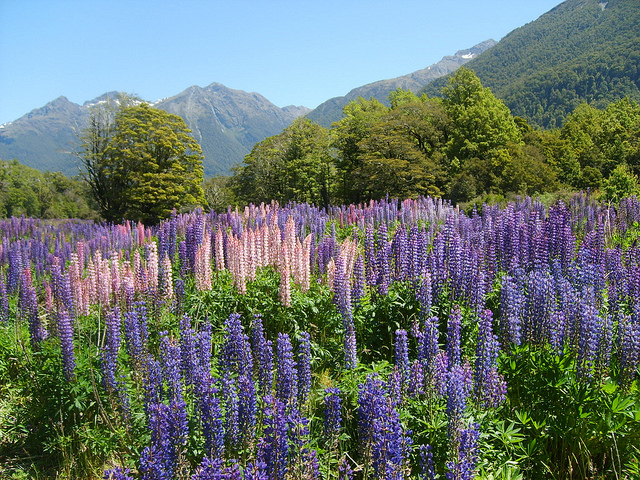
\includegraphics[height =5in]{./Plots/nature.jpg}
	\caption{An individual figure!}
\end{figure*}
        
\begin{figure*}[h]
	\subfloat[\label{fig:HD8538_ellplot}]{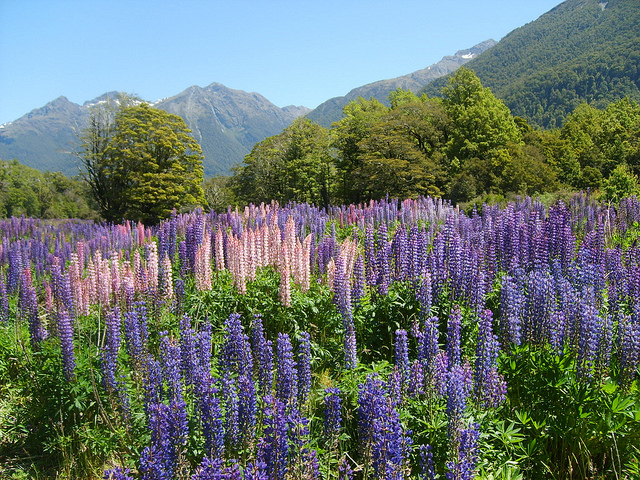
\includegraphics[height =2.5in]{./Plots/nature.jpg}} 
	\subfloat[\label{fig:HD8538_phot}]{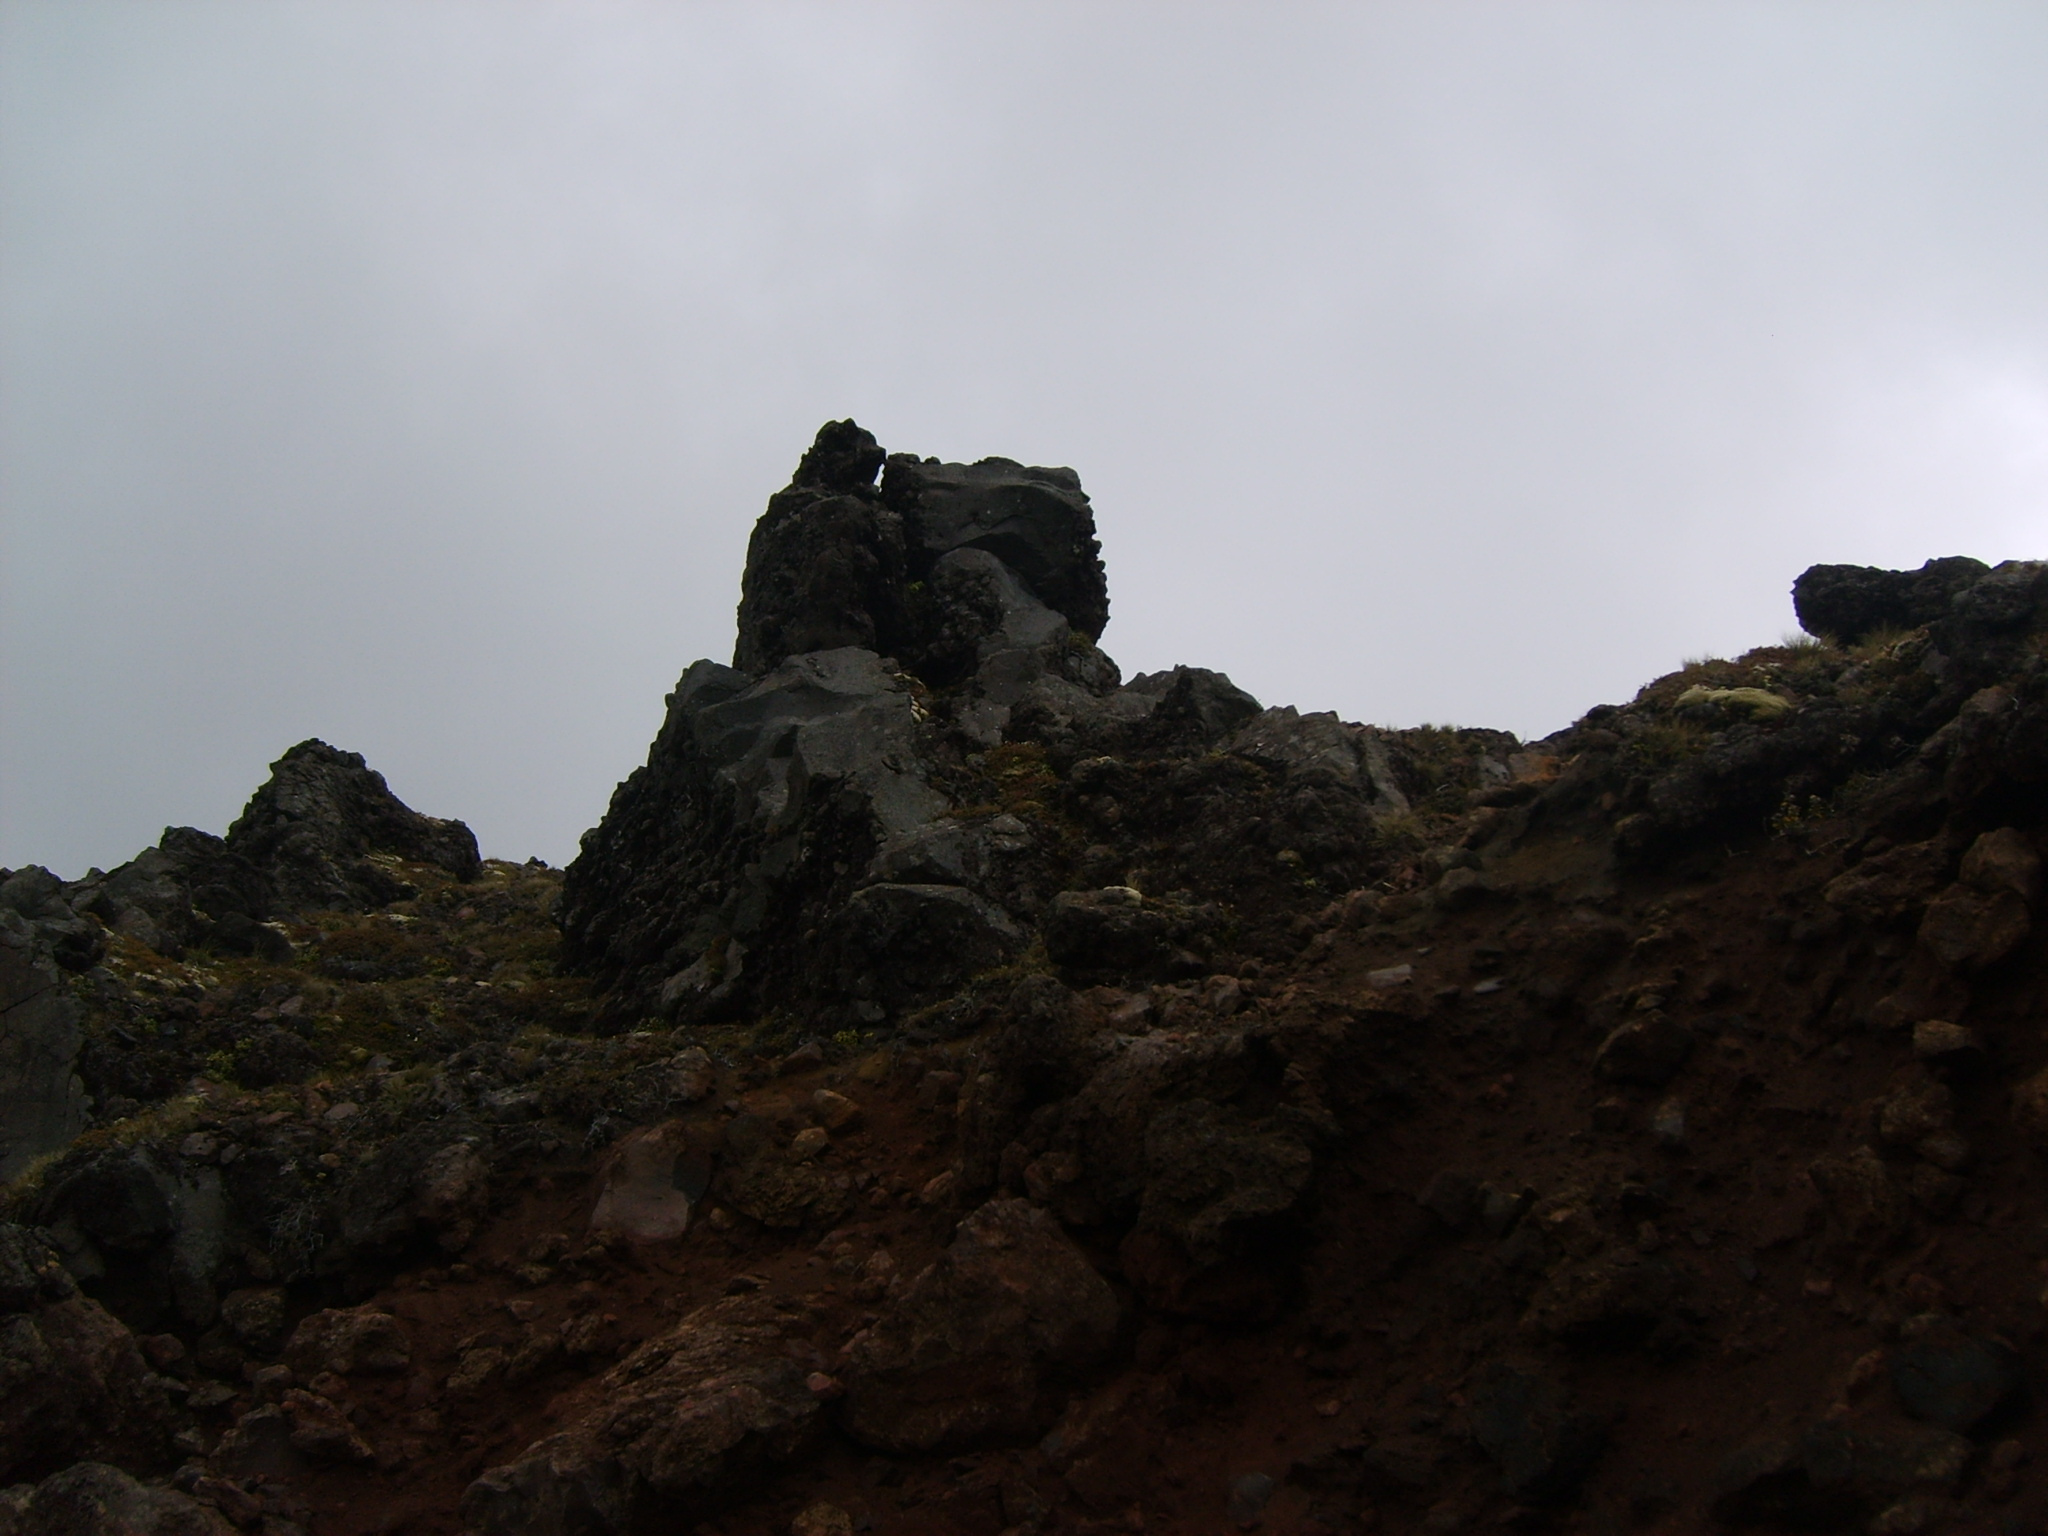
\includegraphics[height =2.5in]{./Plots/rocks.jpg}} \\
	\subfloat[\label{fig:HD8538_vis}]{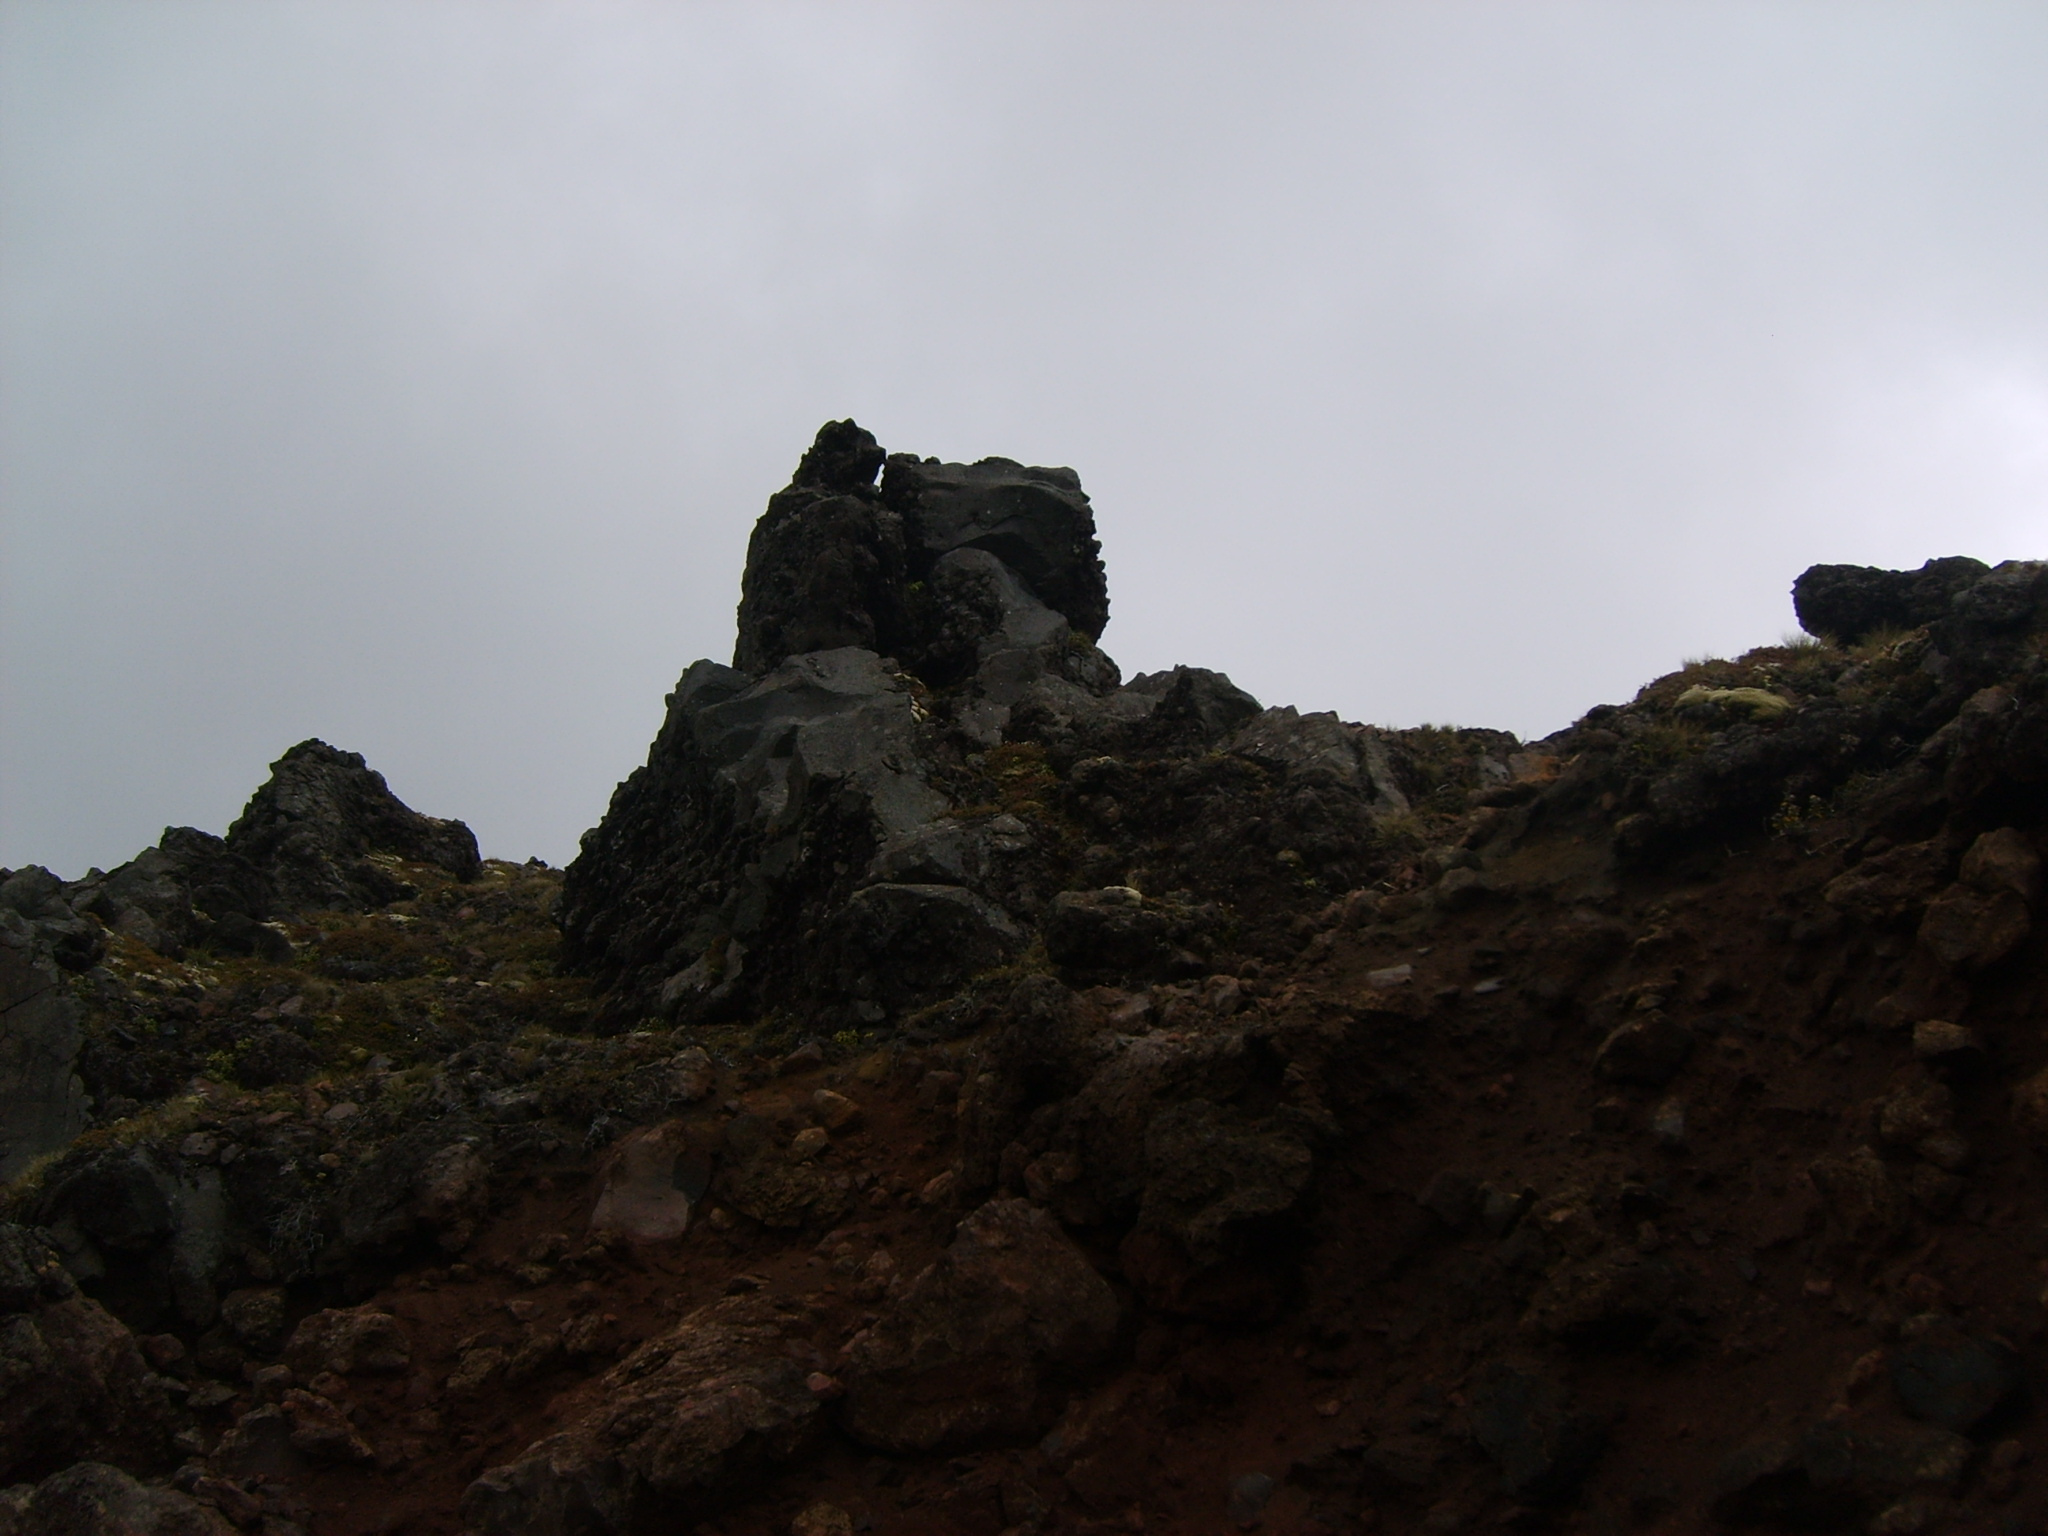
\includegraphics[height =2.5in]{./Plots/rocks.jpg}}
	\subfloat[\label{fig:HD8538_HRD}]{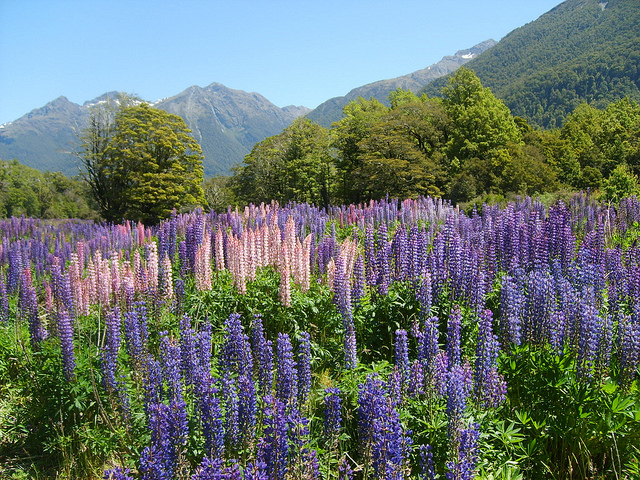
\includegraphics[height =2.5in]{./Plots/nature.jpg}}
	\caption{Multiple figures!}
\end{figure*}



\begin{landscape}
\begin{longtable}{cccccccccccccc}
\label{tab:disk}\\
\caption{Insert Table Caption here}\\
\hline\endhead  % header material
\hline\endfoot  % footer material
\hline
Blah & Blah & Blah \\
\hline
Stuff & Things & etc. \\
\nodata & \nodata & \nodata \\
\end{longtable}
\end{landscape}

\chapter{METHODOLOGY AND ALGORITHM DESCRIPTION}
\newtheorem{lemma}[theorem]{Lemma}
\section{Spectral Transformation}
In this chapter, we shall present a detailed description of the methodologies and implementation of algorithms used in this thesis to solve the generalized eigenvalue problem. We begin by describing the problem setup, followed by a discussion of the algorithms used, together with their implementation details. This chapter aims to provide a comprehensive understanding of how these algorithms are applied to derive the solutions to the problem at hand. We shall also give a description of the numerical experiments we setup to investigate the efficiency of these algorithms.\\
Consider the symmetric-definite generalized eigenvalue problem:
\begin{equation}\label{3.1}
	A\mathbf{v} = \lambda B\mathbf{v}, \qquad \mathbf{v} \neq 0
\end{equation}
where $A$ and $B$ are $m \times m$ real, sparse, symmetric and $B$ is positive definite or positive semi-definite.\\
Problem (\ref{3.1}) can be reformulated  as
\begin{equation}\label{3.2}
	\beta A\mathbf{v} = \alpha B\mathbf{v}, \qquad \mathbf{v} \neq 0
\end{equation}
We have replaced $\lambda$ with $\alpha/\beta$ for convenience so that the generalized eigenvalues will be of the form $(\alpha, \beta)$. If $ \beta = 0$, then the generalized eigenvalues $\Lambda(A, B)$ will be infinite. The formulation using equation(\ref{3.2}) is useful when describing the error bounds, as we shall later see. We shall alternate between (\ref{3.1}) and (\ref{3.2}) when convenient. We also observe that the symmetric-definite generalized eigenvalue problem have real eigenvalues.\\
To compute the eigenvalues and eigenvectors that satisfy equation(\ref{3.1}) with spectral transformation lanczos algorithm, our approach will be in two steps:
\begin{itemize}
	\item[$\bullet$] Transform the generalized problem into a spectral transformed standard eigenvalue problem.
	\item[$\bullet$] Solve the spectral problem with Lanczos algorithm.
\end{itemize}
Let $\sigma \in \mathbb{R}$ be a desired shift such that $A - \sigma B$ is non-singular. The shifted problem takes the form:
\begin{equation}\label{3.3}
	(A - \sigma B)v = (\lambda - \sigma)Bv
\end{equation}
We shall begin by computing decompositions for $A - \sigma B$ and $B$. If $B$ is positive  definite, we can compute a Cholesky decomposition $B = C_bC_b^T$ using SciPy \texttt{cholesky} method which calls LAPACK \textbf{\texttt{xPOTRF}}. However, if $B$ is semi positive definite, this function call fails and we use the more robust pivoted Cholesky factorization \textbf{\texttt{xPSTRF}} by calling the inbuilt LAPACK bindings in SciPy.\\
There are various possible factorization options for $A-\sigma B$. One option is to use the pivoted $LDL^{T}$ factorization used by Michael Stewart(2024) and Thomas Ericsson (1960) where $D$ is a block diagonal matrix with $1 \times 1$ and $2 \times 2$ on the diagonal, and $L$ is a lower triangular matrix. This factorization uses the Bunch-Kaufman pivoting scheme with "rook pivoting" which is stable. Although the standard $LDL^T$ factorization (without "rook pivoting") is available in SciPy linear algebra module, there is no option to use the rook pivoting scheme except if one chooses to write a custom LAPACK binding that makes use of \textbf{\texttt{DSYTRF\_ROOK}}. While this can guarantee some stability for the problem we are trying to solve, it usually involves extra work in processing the $2 \times 2$ blocks to make $D$ diagonal.\\
Another factorization is an eigenvalue decomposition of $A - \sigma B$. If we use a symmetric eigenvalue decomposition $A- \sigma B = UDU^T$, our numerical experiments reveals that this stabilizes the Ritz residuals and generalized form of the residuals together with the advantage that these residuals are insensitive to the conditioning of $A$ and $B$. This can be done using inbuilt eigenvalue solvers in SciPy or any linear algebra library. This is the most promising factorization, however computing eigenvalue decompositions for large problems become computationally expensive and not feasible in reality.

Lastly, we can make use of an $LU$ factorization for $A-\sigma B$. Unlike the previous factorizations, the stability for the Ritz residuals is not as great, as we observe that they depend on the conditioning of $A$ and $B$. However, for the purpose of this thesis, we make use of the $LU$ decomposition since it is computationally less expensive and easy to use and implement.

One major takeaway from our experiments with the various options of factorizing $A-\sigma B$ is that symmetry is clearly important for stability. We plan to give a mathematical justification for this in future work.

Continuing with the algorithm derivation, if we assume $\lambda \neq \infty$ and $\mathbf{v} \neq \mathbf{0}$. Since $B$ is positive definite, Michael Stewart (2024), proved that we can compute a Cholesky factorization $B = C_bC_b^T$, and apply the shift-invert spectral transformation to transform equation(\ref{3.1}) into its spectral form as described in section (\ref{section-2.11}) such that $\theta = 1/(\lambda - \sigma)$ is an eigenvalue of the problem :
\begin{equation}\label{3.4}
	C_b^T (A-\sigma B)^{-1} C_b \mathbf{u} = \theta \mathbf{u}, \qquad \mathbf{u} \neq \mathbf{0}
\end{equation}
where  $\mathbf{u} = C_b^T \mathbf{v} \neq \mathbf{0}.$\\
Conversely, assume that $\mathbf{u} \neq \mathbf{0}$ is an eigenvector of (\ref{3.4}) and $\theta$ its corresponding eigenvalue, then the vector $v = (A-\sigma B)^{-1}C_b \mathbf{u} \neq \mathbf{0}$ is an eigenvector for (\ref{3.2}), with eigenvalue $(1+\sigma \theta, \theta)$, provided $C_b\mathbf{u} \neq \mathbf{0}$.\\[10pt]
Equation (\ref{3.4}) gives us the spectral transformed version of the original generalized problem. Since the problem is now in a standard form, we can then apply the Lanczos algorithm to compute the desired eigenvalues within the neighborhood of $\sigma$, together with their corresponding eigenvectors. It should be noted that forming the spectral matrix in (\ref{3.4}) is not desirable as it will make the Lanczos algorithm unstable. Forming the matrix directly also has the disadvantage that the matrix might no longer be symmetric which could prevent the Lanczos algorithm from converging. The right thing to do is to use the $LU$ for $A-\sigma B$ as explained earlier. This will be explored in the next section.
\section{Lanczos decomposition}
In this section, we revisit the Lanczos algorithm, and discuss how we apply it to the spectral transformed problem. As discussed in section \ref{section2.10}, the Lanczos algorithm approximates the eigenvalues of the original problem by projecting it onto a Krylov subspace spanned by successive powers of the system matrix applied to an initial vector. The eigenvalues approximation arises from the tridiagonal matrix obtained through the Lanczos process, which captures the essential spectral characteristics of the original matrix.\\
Given $A \in \mathbb{R}^{m \times m}$, with $A=A^T$, the pesudocode for the lanczos algorithm is given as follows:
\begin{algorithm}
	\caption{Lanczos Algorithm for a Symmetric Matrix}
	\label{alg:lanczos_algorithm}

	\textbf{Require:} \( A = A^T \), number of iterations: \(n\), tolerance: \(tol\)
	\begin{algorithmic}[1]
		\Function{lanczos}{$A, n, tol$}
		\State Choose an arbitrary vector $b$ and set an initial vector $q_1 = b/ \|b\|_2$ 
		\State Set $\beta_0 = 0$ and $q_0 = 0$
			\For{$j = 1, 2, \dots, n$}
		\State $v = A q_j$
		\State $\alpha_j = q_j^T v $
		\State $v = v - \beta_{j-1}q_{j-1} - \alpha_j q_j$
		\State \textbf{Full reorthogonalization:} $v = v - \sum_{i \leq j} (q_i^T v) q_i$
		\State $\beta_{j} = \|v\|_2$
		\If{$\beta_{j} < tol $}
		\State \textbf{restart} or \textbf{exit}
		\EndIf
		\State $q_{j+1} := v / \beta_{j}$
		\EndFor
		\EndFunction
	\end{algorithmic}
\end{algorithm}\\
After the completion of algorithm \ref{alg:lanczos_algorithm}, the $\alpha$'s and $\beta$'s are used to construct the tridiagonal matrix $T_n \in \mathbb{R}^{n \times n}$ and the vectors $q_j$'s are stacked together to form an orthogonal matrix $Q_n \in \mathbb{R}^{m \times n}$ given by:
\[T_n = \begin{pmatrix}
			\alpha_1 & \beta_1 & & & \\\beta_1 & \alpha_2 & \beta_2 & & \\ & \beta_2 & \alpha_3 & \beta_3 & \\ & & \ddots & \ddots & \vdots \\ & & & \beta_{n-1} & \alpha_n
		\end{pmatrix}\] 
	\[
	Q_n = 
	\begin{bmatrix}
		 & \big| &  & \big| &  & \big| &  \\
		 & \big| &  & \big| &  & \big| &  \\
		 q_1 & \big| & q_2 & \big| & \cdots & \big| & q_n \\
		 & \big| &  & \big| &  & \big| &  \\
		 & \big| &  & \big| &  & \big| &  \\
	\end{bmatrix}.
	\]
The decomposition is given by
\begin{equation}
	AQ_n = Q_nT_n + \beta_{n}q_{n+1}e_n^T
\end{equation}
In theory, the vectors $q_j$'s should be orthonormal, but due to floating-point errors, there will be loss of orthogonalization, hence the need for line 8 in the Algorithm \ref{alg:lanczos_algorithm}.\\
Let $\theta_i, i = 1,2, \ldots n$(which can be computed by standard functions in using any eigenvalue solver) be the eigenvalues of $T_n$, and $\{y_i\}_{i = 1 : n}$ be the associated eigenvectors. The $\{\theta_i\}$ are called the \textit{Ritz values} and the vectors $\{Q_ny_i\}_{i = 1 : n}$ are called the \textit{Ritz vectors}. Hence, the eigenvalues of $A$ are on both ends of the are well approximated by the Ritz values, with the Ritz vectors as their approximate corresponding eigenvectors of $A$.\par
Since the generalized eigenvalue problem we started with has been reduced to a standard one as shown in equation (\ref{3.3}), Algorithm (\ref{alg:lanczos_algorithm}) can be applied to equation (\ref{3.3}) with some slight modifications. We shall now give the spectral form of Algorithm (\ref{alg:lanczos_algorithm}):\\
\begin{algorithm}
	\caption{Spectral Lanczos Algorithm for (\ref{3.4}) }
	\label{alg:spectral_lanczos_algorithm}
	
	\textbf{Require:} \( A = A^T \), \( B = B^T \), with \(B\) being positive definite or semidefinite\\
	\textbf{Require:} number of iterations: \(n\), size of matrix $A$ or $B$: $m$, tolerance: \(tol\)\\
	\textbf{Require:} \(\sigma \in \mathbb{R}\): shift not close to a generalized eigenvalue
	\begin{algorithmic}[1]
		\Function{\textsc{Spectral\_Lanczos}}{$A, B, m, n, \sigma, tol$}
		\State Choose an arbitrary vector $b$ and set an initial vector $q_1 = b/ \|b\|_2$
		\State Set $\beta_0 = 0$ and $q_0 = 0$
		\State Set $Q = zeros(m, n+1)$
		\State Precompute the $LU$ factorization of $A - \sigma B$: $LU = (A - \sigma B)$
		\State Factor: $B = CC^T$
		\For{$j = 1, 2, \dots, n$}
		\State $Q[:, j] = q_j$
		\State $u = Cq_j$
		\State Solve: $(LU)v = u$ for $v$
		\State $v = C^T v$
		\If{$j < n $}
		\State $\alpha_j = q_j^T v $
		\State $v = v - \beta_{j-1}q_{j-1} - \alpha_j q_j$
		\State \textbf{Full reorthogonalization:} $v = v - \sum_{i \leq j} (q_i^T v) q_i$
		\State $\beta_{j} = \|v\|_2$
		\If{$\beta_{j} < tol $}
		\State \textbf{restart} or \textbf{exit}
		\EndIf
		\State $q_{j+1} := v / \beta_{j}$
		\EndIf
		\EndFor
		\State $Q = Q[:, :n]$
		\State $q = Q[:, n]$
		\State \Return $(Q, T, q)$
		\EndFunction
	\end{algorithmic}
\end{algorithm}\\
After applying the lanczos procedure to the spectral transformed problem (\ref{3.4}), we then compute the converged Ritz pairs using a certain tolerance. The converged Ritz pairs are mapped to the generalized eigenvalues and eigenvectors where we can observe the behaviour of these residuals with respect to conditioning.
\section{Experimental Setup}
To evaluate the performance and robustness of the spectral transformation lanczos algorithm, we setup a problem with predetermined eigenvalues, use the algorithm to compute the eigenvalues, and show that the residuals follow closely with the bounds predicted by direct methods. While there are other options of using matrices from open source repositories like Matrix Market, we choose to use this approach so that we can control the size, condition number and other properties of the matrix so as to observe the effect of this properties on the algorithm.

Starting with a diagonal matrix $D \in \mathbb{R}^{m \times m}$ with known eigenvalues, we generate a random matrix $P$ of size $m \times m $ with standard normal distribution. Since the $QR$ factorization is guaranteed to exist for any matrix, we take the $QR$ factorization of $P$ to obtain an orthogonal matrix $Q$, which is used to create a matrix $C$ using orthogonal transformation. Hence $C = QDQ^T$ is unitarily similar to $D$.

Next, we initialize a random lower triangular matrix $L_0 \in \mathbb{R}^{m \times m}$ with a normal distribution. A symmetric positive definite $B \in \mathbb{R}$ is formed by
\begin{equation}
	B = L_0 L_0^T + \delta I_m, \qquad \delta > 0
\end{equation}
where $I_m$ is an identity matrix of order $m$. Clearly, $B$ is symmetric. The matrix $L_0L_0^T$ is positive semi-definite since for any non-zero vector $\mathbf{x}$
\begin{equation}
	\mathbf{x}^T(L_0L_0^T)\mathbf{x} = (L_0^T\mathbf{x})^T(L_0^T\mathbf{x}) = \| L_0^T\mathbf{x} \|^2 \geq \mathbf{0}
\end{equation}
However, $L_0L_0^T$ may not be strictly positive definite if $L_0$ is singular. The term $\delta I_m$ ensures strict positve definiteness by adding $\delta$ to its diagonals, thereby shifting all eigenvalues by $\delta$. If $\delta > 0$, then all eigenvalues of $B$ will be strictly positive, ensuring $B$ is positive definite. This guarantees that we can compute the Cholesky factorization of $B$ without any numerical issues.

Another important thing to note is that, $\delta$ can be used to control the conditioning of $B$. We recall from section (\ref{section1.2.6}), that the condition number of $B$ when $B$ is symmetric, is defined as:
\begin{equation}
	\kappa(B) = \frac{\lambda_{\max}(B)}{\lambda_{\min}(B)}
\end{equation}
where $\lambda_{\max}(B)$ and $\lambda_{\min}(B)$ are the largest and smallest eigenvalues of B, respectively.
In general, $B$ is usually ill-conditioned with a very large condition number so that if $\delta$ is large, the process of adding $\delta I_m$ can regularize the condition number of $B$, making $B$ well-conditioned, since that will equate to increasing $\lambda_{\min}(B)$. If delta is small, $B$ can still be ill-conditioned but not in an astronomical way. Hence, $\delta$ is a hyperparameter we can use to control the condition of $B$. In this experiment, we choose $\delta = 10^{-2}$, which gives a condition number of $\kappa(B) = 5.39 \times 10^5$.\\
Since $B$ is symmetric and positive definite, we can compute it's Cholesky factorization $B = LL^T$ and construct $A$ using a congruence transformation
\begin{equation}\label{3.9}
	A = LCL^T
\end{equation}
So that the generalized eigenvalues $\Lambda(A, B)$ is equal to the eigenvalues of the diagonal matrix $D$. This can be summarized by the following lemma:
\begin{lemma}
	Let $A-\lambda B$ be a pencil, where $A$ and $B$ are symmetric, and $B$ is strictly positive definite. Let $D$ be a diagonal matrix and $C$ be unitarily similar to $D$. Assuming (\ref{3.9}) holds, then the generalized eigenvalues $\Lambda(A, B)$ is similar to $D$
\end{lemma}

\begin{proof}
	Given the generalized problem
	\begin{equation}
		A \mathbf{v} = \lambda B \mathbf{v}, \qquad \mathbf{v} \neq \mathbf{0}
	\end{equation}
	Since $B$ is positive definite, then clearly, it is invertible and the generalized eigenvalues $\Lambda(A, B)$ will be the eigenvalues of $B^{-1}A$.\\
	Now
	\begin{align*}
		B^{-1}A & = (LL^T)^{-1}(LCL^T)\\
		& = L^{-T}L^{-1}LQDQ^{T}L^T\\
		& = (L^{-T}Q)D(Q^{-1}L^{T}) \\
		& = (L^{-T}Q)D(L^{-T}Q)^{-1}
	\end{align*}
	Therefore $B^{-1}A$ is similar to $D$ and hence $\Lambda(A,B)$ is similar to $D$.
\end{proof}
The pseudocode for generating $A$ and $B$ is given as follows:
\begin{algorithm}
	\caption{Setting up a GEP}
	\label{alg:problem setup}
	
	\textbf{Require:} \( D \): diagonal matrix with known eigenvalues, \(\delta\): regularization hyperparameter
	\begin{algorithmic}[1]
		\Function{\textsc{Generate\_Matrix}}{$D, \delta$}
		\State Set $m$ = \texttt{size}($D$)
		\State $Q$, \_\_ = \texttt{qr}(random.randn($m$, $m$))
		\State $C = QDQ^T$
		\State $L_{0}$ = \texttt{tril}(\texttt{random.randn}($m$, $m$))
		\State $B = (L_0 L_0^T) + \delta \cdot eye (m)$
		\State $L$ = \texttt{cholesky}($B$)
		\State $A$ = $LCL^T$
		\State \Return ($A$, $B$)
		\EndFunction
	\end{algorithmic}
\end{algorithm}\\
With the problem setup completed, and the algorithm described, in the next chapter, we shall discuss the results obtained in these experiments.























\chapter{CONCLUSION}
This thesis has investigated the application and performance of the Spectral Transformation Lanczos algorithm for solving symmetric definite dense generalized eigenvalue problem. Through the numerical experiments, we validated our results with proven error bounds in direct methods, considered the implication of several methods, and the impact of certain properties of the matrix on the accuracy of the results. In this concluding chapter, we summarize our key findings, discuss the broader implications of this work, acknowledge limitations, and outline promising directions for future research.

\section{Summary of Key Findings}
The experiments in this thesis have uncovered some interesting results regarding the spectral transformation lanczos algorithm for generalized eigenvalue problems. First, we have established that the generalized residuals increases for eigenvalues farther away from the shift, if the shift is not too large in magnitude, validating the analytical error bounds proven for direct methods.\\[10pt]
Secondly, our analysis of the eigenvalue sensitivity revealed the relationship between the conditioning of the matrices, and the accuracy of computed eigenvalues for various factorizations of the shifted matrix $A-\sigma B$. We observed that for any factorization involving symmetry(eigenvalue decomposition or $LDL^T$ factorization), the ST-Lanczos is stable and the Ritz pairs converged to the order of unit round off $u$ for the $n-$ lanczos steps. The generalized eigenvalues also converged, achieving unit round off for all computed eigenvalues closer and farther away from the shift. This poses an interesting question: ``Can we prove stability for any symmetric decomposition of $A - \sigma B$''?

Finally, for the $LU$ decomposition of $A - \sigma B$, we observe that the lanczos procedure was stable but the behavior is largely dependent on the conditioning of \rep{$A-\sigma B$}{$A$ and $B$}. However, our results indicated that, the generalized residuals were insensitive to the conditioning of the problem.

\section{Importance and Implications}
From a theoretical perspective, this work advances our knowledge of spectral transformation, matrix conditioning and eigenvalue sensitivity in the context of dense generalized eigenvalue problems. Our results showed that the conditional bounds for direct methods, holds true for iterative methods. This work goes a step further at highlighting an interesting property of spectral transformation methods that can determine stability for such methods, both in the direct and iterative context. This contributes to the broader field of numerical linear algebra by providing a more comprehensive framework for analyzing iterative eigenvalue solvers.

By characterizing the relationship between matrix factorizations and algorithm convergence, we have developed a better understanding of how spectral transformations affect the convergence of properties of Krylov subspace methods.



%%% Local Variables:
%%% mode: LaTeX
%%% TeX-master: "../main"
%%% End:





%%%%%%%%%%%%%%%%%%%% The backmatter goes in this file %%%%%%%%%%%%%%%%%%%%%

% The bibliography starts here.

\bibliographystyle{apj}             % Please learn to use the
                                    % formatting of Latex's Bibtex. It
                                    % will make your life easier.

\bibliography{bibliography}
%\bibliography{apj-jour,dissref}       % "paper.bib" contains all my
                                    % references. "apj-jour.bib"
                                    % contains abbreviations of
                                    % journals.


\clearpage
% If you have only one appendix chapter, use the command
% \begin{appendix}...\end{appendix} instead.
% This takes care of the requirement (of the Graduate Office) for one
% appendix chapter to be labeled as 'Appendix', not 'Appendix A'.

\beforechapterheadname{APPENDIX}         % Optional text to put in front of
                                   % the chapter number.
\afterchapterheadname{}          % Optional text to put after the

\addcontentsline{toc}{chapter}{APPENDIX}

%\begin{appendix}
%  \input{appendixI}                     % Your appendices go here.
%  %%
%% This is file `appendix.sty',
%% generated with the docstrip utility.
%%
%% The original source files were:
%%
%% appendix.dtx  (with options: `usc')
%%
%% -----------------------------------------------------------------
%%   Author: Peter Wilson (CUA) now at peter.r.wilson@boeing.com until June 2004
%%                              (or at: pandgwilson at earthlink dot net)
%%   Copyright 1998 --- 2004 Peter R. Wilson
%%
%%   This work may be distributed and/or modified under the
%%   conditions of the LaTeX Project Public License, either
%%   version 1.3 of this license or (at your option) any
%%   later version.
%%   The latest version of the license is in
%%      http://www.latex-project.org/lppl.txt
%%   and version 1.3 or later is part of all distributions of
%%   LaTeX version 2003/06/01 or later.
%%
%%   This work has the LPPL maintenance status "author-maintained".
%%
%%   This work consists of the files listed in the README file.
%% -----------------------------------------------------------------
%%
\NeedsTeXFormat{LaTeX2e}
\ProvidesPackage{appendix}[2002/08/06 v1.2 extra appendix facilities]

\newif\if@chapter@pp\@chapter@ppfalse
\newif\if@knownclass@pp\@knownclass@ppfalse
\@ifundefined{chapter}{%
  \@ifundefined{section}{}{\@knownclass@pptrue}}{%
  \@chapter@pptrue\@knownclass@pptrue}
\providecommand{\phantomsection}{}
\newcounter{@pps}
  \renewcommand{\the@pps}{\alph{@pps}}
\newif\if@pphyper
  \@pphyperfalse
\AtBeginDocument{%
  \@ifpackageloaded{hyperref}{\@pphypertrue}{}}

\newif\if@dotoc@pp\@dotoc@ppfalse
\newif\if@dotitle@pp\@dotitle@ppfalse
\newif\if@dotitletoc@pp\@dotitletoc@ppfalse
\newif\if@dohead@pp\@dohead@ppfalse
\newif\if@dopage@pp\@dopage@ppfalse
\DeclareOption{toc}{\@dotoc@pptrue}
\DeclareOption{title}{\@dotitle@pptrue}
\DeclareOption{titletoc}{\@dotitletoc@pptrue}
\DeclareOption{header}{\@dohead@pptrue}
\DeclareOption{page}{\@dopage@pptrue}
\ProcessOptions\relax
\newcommand{\@ppendinput}{}
\if@knownclass@pp\else
  \PackageWarningNoLine{appendix}%
    {There is no \protect\chapter\space or \protect\section\space command.\MessageBreak
     The appendix package will not be used}
  \renewcommand{\@ppendinput}{\endinput}
\fi
\@ppendinput

\newcommand{\appendixtocon}{\@dotoc@pptrue}
\newcommand{\appendixtocoff}{\@dotoc@ppfalse}
\newcommand{\appendixpageon}{\@dopage@pptrue}
\newcommand{\appendixpageoff}{\@dopage@ppfalse}
\newcommand{\appendixtitleon}{\@dotitle@pptrue}
\newcommand{\appendixtitleoff}{\@dotitle@ppfalse}
\newcommand{\appendixtitletocon}{\@dotitletoc@pptrue}
\newcommand{\appendixtitletocoff}{\@dotitletoc@ppfalse}
\newcommand{\appendixheaderon}{\@dohead@pptrue}
\newcommand{\appendixheaderoff}{\@dohead@ppfalse}
\newcounter{@ppsavesec}
\newcounter{@ppsaveapp}
\setcounter{@ppsaveapp}{0}
\newcommand{\@ppsavesec}{%
  \if@chapter@pp \setcounter{@ppsavesec}{\value{chapter}} \else
                 \setcounter{@ppsavesec}{\value{section}} \fi}
\newcommand{\@pprestoresec}{%
  \if@chapter@pp \setcounter{chapter}{\value{@ppsavesec}} \else
                 \setcounter{section}{\value{@ppsavesec}} \fi}
\newcommand{\@ppsaveapp}{%
  \if@chapter@pp \setcounter{@ppsaveapp}{\value{chapter}} \else
                 \setcounter{@ppsaveapp}{\value{section}} \fi}
\newcommand{\restoreapp}{%
  \if@chapter@pp \setcounter{chapter}{\value{@ppsaveapp}} \else
                 \setcounter{section}{\value{@ppsaveapp}} \fi}
\providecommand{\appendixname}{APPENDIX}
\newcommand{\appendixtocname}{APPENDICES}
\newcommand{\appendixpagename}{APPENDICES}
\newcommand{\appendixpage}{%
%  \if@chapter@pp \@chap@pppage \else \@sec@pppage \fi
  \if@chapter@pp \else \@sec@pppage \fi
}
\newcommand{\clear@ppage}{%
  \if@openright\cleardoublepage\else\clearpage\fi}

\newcommand{\@chap@pppage}{%
%  \clear@ppage
%  \thispagestyle{plain}%
  \if@twocolumn\onecolumn\@tempswatrue\else\@tempswafalse\fi
%  \null\vfil
%  \markboth{}{}%
  {\centering
%   \interlinepenalty \@M
   \normalfont
   \normalsize \bfseries \appendixpagename\par}%
  \if@dotoc@pp
    \addappheadtotoc
  \fi
  \vfil%\newpage
  \if@twoside
    \if@openright
%      \null
%      \thispagestyle{empty}%
      %\newpage
    \fi
  \fi
  \if@tempswa
    \twocolumn
  \fi
}

\newcommand{\@sec@pppage}{%
  \par
  \addvspace{4ex}%
  \@afterindentfalse
  {\parindent \z@ \raggedright
   \interlinepenalty \@M
   \normalfont
   \normalsize \bfseries \appendixpagename%
   \markboth{}{}\par}%
  \if@dotoc@pp
    \addappheadtotoc
  \fi
  \nobreak
  \vskip 3ex
  \@afterheading
}

\newif\if@pptocpage
  \@pptocpagetrue
\newcommand{\noappendicestocpagenum}{\@pptocpagefalse}
\newcommand{\appendicestocpagenum}{\@pptocpagetrue}
\newcommand{\addappheadtotoc}{%
  \phantomsection
  \if@chapter@pp
    \if@pptocpage
      \addcontentsline{toc}{chapter}{\appendixtocname}%
    \else
      \if@pphyper
        \addtocontents{toc}%
          {\protect\contentsline{chapter}{\appendixtocname}{}{\@currentHref}}%
      \else
        \addtocontents{toc}%
          {\protect\contentsline{chapter}{\appendixtocname}{}}%
      \fi
    \fi
  \else
    \if@pptocpage
      \addcontentsline{toc}{section}{\appendixtocname}%
    \else
      \if@pphyper
        \addtocontents{toc}%
          {\protect\contentsline{section}{\appendixtocname}{}{\@currentHref}}%
      \else
        \addtocontents{toc}%
          {\protect\contentsline{section}{\appendixtocname}{}}%
      \fi
    \fi
  \fi
}

\providecommand{\theH@pps}{\alph{@pps}}

\newcommand{\@resets@pp}{\par
  \@ppsavesec
  \stepcounter{@pps}
  \setcounter{section}{0}%
  \if@chapter@pp
    \setcounter{chapter}{0}%
    \renewcommand\@chapapp{\appendixname}%
     \ifthenelse{\equal{\thechapter}{}}{\renewcommand\thesection{\@Alph\c@section}}{\renewcommand\thechapter{\@Alph\c@chapter}}
  \else
    \setcounter{subsection}{0}%
    \renewcommand\thesection{\@Alph\c@section}%
  \fi
  \if@pphyper
    \if@chapter@pp
      \renewcommand{\theHchapter}{\theH@pps.\Alph{chapter}}%
    \else
      \renewcommand{\theHsection}{\theH@pps.\Alph{section}}%
    \fi
    \def\Hy@chapapp{\appendixname}%
  \fi
  \restoreapp
}

\newenvironment{appendices}{%
  \@resets@pp
  \if@dotoc@pp
    \if@dopage@pp              % both page and toc
      \if@chapter@pp           % chapters
%        \clear@ppage
      \fi
      \appendixpage
    \else                      % toc only
       \if@chapter@pp          % chapters
%         \clear@ppage
       \fi
      \addappheadtotoc
    \fi
  \else
    \if@dopage@pp              % page only
      \appendixpage
    \fi
  \fi
  \if@chapter@pp
    \if@dotitletoc@pp \@redotocentry@pp{chapter} \fi
  \else
    \if@dotitletoc@pp \@redotocentry@pp{section} \fi
    \if@dohead@pp
      \def\sectionmark##1{%
        \if@twoside
          \markboth{\@formatsecmark@pp{##1}}{}
        \else
          \markright{\@formatsecmark@pp{##1}}{}
        \fi}
    \fi
    \if@dotitle@pp
      \def\sectionname{\appendixname}
      \def\@seccntformat##1{\@ifundefined{##1name}{}{\csname ##1name\endcsname\ }%
        \csname the##1\endcsname\quad}
    \fi
  \fi}{%
  \@ppsaveapp\@pprestoresec}

\newcommand{\setthesection}{\thechapter.\Alph{section}}
\newcommand{\setthesubsection}{\thesection.\Alph{subsection}}

\newcommand{\@resets@ppsub}{\par
  \stepcounter{@pps}
  \if@chapter@pp
    \setcounter{section}{0}
    \renewcommand{\thesection}{\setthesection}
  \else
    \setcounter{subsection}{0}
    \renewcommand{\thesubsection}{\setthesubsection}
  \fi
  \if@pphyper
    \if@chapter@pp
      \renewcommand{\theHsection}{\theH@pps.\setthesection}%
    \else
      \renewcommand{\theHsubsection}{\theH@pps.\setthesubsection}%
    \fi
    \def\Hy@chapapp{\appendixname}%
  \fi
}

\newenvironment{subappendices}{%
  \@resets@ppsub
  \if@chapter@pp
    \if@dotitletoc@pp \@redotocentry@pp{section} \fi
    \if@dotitle@pp
      \def\sectionname{\appendixname}
      \def\@seccntformat##1{\@ifundefined{##1name}{}{\csname ##1name\endcsname\ }%
        \csname the##1\endcsname\quad}
    \fi
  \else
    \if@dotitletoc@pp \@redotocentry@pp{subsection} \fi
    \if@dotitle@pp
      \def\subsectionname{\appendixname}
      \def\@seccntformat##1{\@ifundefined{##1name}{}{\csname ##1name\endcsname\ }%
        \csname the##1\endcsname\quad}
    \fi
  \fi}{}

\newcommand{\@formatsecmark@pp}[1]{%
  \MakeUppercase{\appendixname\space
    \ifnum \c@secnumdepth >\z@
      \thesection\quad
    \fi
    #1}}
\newcommand{\@redotocentry@pp}[1]{%
  \let\oldacl@pp=\addcontentsline
  \def\addcontentsline##1##2##3{%
    \def\@pptempa{##1}\def\@pptempb{toc}%
    \ifx\@pptempa\@pptempb
      \def\@pptempa{##2}\def\@pptempb{#1}%
      \ifx\@pptempa\@pptempb
\oldacl@pp{##1}{##2}{\appendixname\space ##3}%
      \else
        \oldacl@pp{##1}{##2}{##3}%
      \fi
    \else
      \oldacl@pp{##1}{##2}{##3}%
    \fi}
}

\endinput
%%
%% End of file `appendix.sty'.
                     %named "appendix.tex"
%\end{appendix}
               % See the backmatter.tex file


%%%%%%%%%%%%%%%%%%%%%%%%%%%%%%%%%%%%%%%%%%%%%%%%%%%%%%%%%%%%%%%%%%%%%%
%               The dissertation ends here.                          %
%%%%%%%%%%%%%%%%%%%%%%%%%%%%%%%%%%%%%%%%%%%%%%%%%%%%%%%%%%%%%%%%%%%%%%

\end{document}
